\documentclass[a4paper]{spie}

\renewcommand{\baselinestretch}{1.0} % Change to 1.65 for double spacing
 
\usepackage{amsmath,amsfonts,amssymb}
\usepackage{graphicx}
\usepackage[colorlinks=true, allcolors=blue]{hyperref}

\title{Support Vector Machines for Prostate Lesion Classification in the ProstateX Challenge}

\author[a]{Andy Kitchen}
\author[b]{Jarrel Seah}

\affil[a]{Silverpond Pty. Ltd.,
  2/382 Little Collins Street,
  Melbourne VIC 3000, Australia}
\affil[b]{STAT Innovations Pty. Ltd.,
  PO Box 274, Ashburton VIC 3147,
  Australia}

\authorinfo{Further author information:\\
  Andy Kitchen: E-mail: andy.kitchen@silverpond.com.au, Telephone: +61 432 514 287\\
  Jarrel Seah: E-mail: jarrelscy@gmail.com, Telephone: +61 450 681 551}

% Option to view page numbers
\pagestyle{empty} % change to \pagestyle{plain} for page numbers   
\setcounter{page}{1} % Set start page numbering at e.g. 301

\begin{document} 
\maketitle

\begin{abstract}
Support vector machines (SVM) are applied to the problem of prostate lesion classification for the SPIE ProstateX Challenge 2016, achieving a score of 0.82 AUC on held-out test data. Square 5mm transverse image patches are extracted around each lesion center from aligned MRI scans. Three MRI modalities are simultaneously analyzed: T2-weighted, apparent diffusion coefficient (ADC) and volume transfer constant ($K^{\mathit{trans}}$). Extracted patches are used to train a binary classifier to predict clinical significance.  The machine learning algorithm is trained on 76 positive cases and 254 negative cases (330 total) from the challenge. The method is conceptually simple, trains in a few seconds and yields competitive results.
\end{abstract}

\keywords{ProstateX, MRI, prostate, support vector machine, machine learning, computer-aided diagnosis}

\section{INTRODUCTION}

The Support Vector Machine\cite{CortesVapnik1995} (SVM) is applied to the problem of prostate lesion classification for the SPIE ProstateX Challenge 2016. This machine learning algorithm is trained on MRI scans to classify new unseen lesions as clinically significant or not. The method described achieves competitive performance with a score of 0.82 area under the curve (AUC) assessed on held-out test data with correct answers kept hidden by competition organizers. This approach is conceptually simple. There are no involved processing steps or complex computer vision algorithms. The method is efficient, due to its simplicity and the availability of highly optimized implementations of SVMs. The implementation uses free and open source software tools and libraries, so there are no encumbrances to further research or reproduction; all code is extensible and auditable.

The data provided for the challenge is a collection of patients each with MRI images in multiple modalities and metadata provided as comma separated value (CSV) files. For each patient one or more prostate lesions and their locations have been identified. For patients in the training set, each lesion is labeled with its clinical significance (true or false). The task is to predict the hidden labels for the patients in the test set. Three MRI modalities are simultaneously analyzed by this method: T2-weighted, apparent diffusion coefficient (ADC) and volume transfer constant ($K^{\mathit{trans}}$); which are all shown to be related to clinical significance\cite{langer2010prostate}. These modalities are all aligned and processed together.

\section{METHOD}

\subsection{Preprocessing}

The ProstateX input data is complex, including multiple data structures and formats. Processing and reconciling inconsistent or overlapping metadata is a major challenge. Multiple rules were applied on each patient to heuristically extract the most relevant T2, ADC and $K^{\mathit{trans}}$ images. Metadata was collated from both Comma Separated Value (CSV) files and information embedded within image files themselves. Significant effort was expended in this area, rivaling that spent on machine learning models.

\subsection{Patch Extraction}

For each patient, and each lesion, a centered $5\text{mm} \times 5\text{mm}$ patch is extracted at a resolution of 1px/mm (see figure \ref{figure:patch}) in 3 modalities T2, ADC and $K^{\mathit{trans}}$. Only transverse image slices are used. Images are flattened into 75 ($5 \times 5 \times 3$) dimensional vectors. We further augment this vector with zone information by encoding it as dummy variables\cite{Hastie2009} which are then concatenated with the image vector. See table \ref{table:performance} for performance comparison without zone information.

Patch extraction subroutines were validated using pixel-by-pixel comparison to the reference images released by the challenge organizers and were found to be in close agreement. All processing is internally carried out with 32-bit floating point pixel values. This preserves large dynamic range and subtle contrast differences important for later analysis.

\begin{figure}
\begin{center}
  \caption{T2-weighted MRI image with red rectangle showing patch area with surrounding lesion}
  \label{figure:patch}
  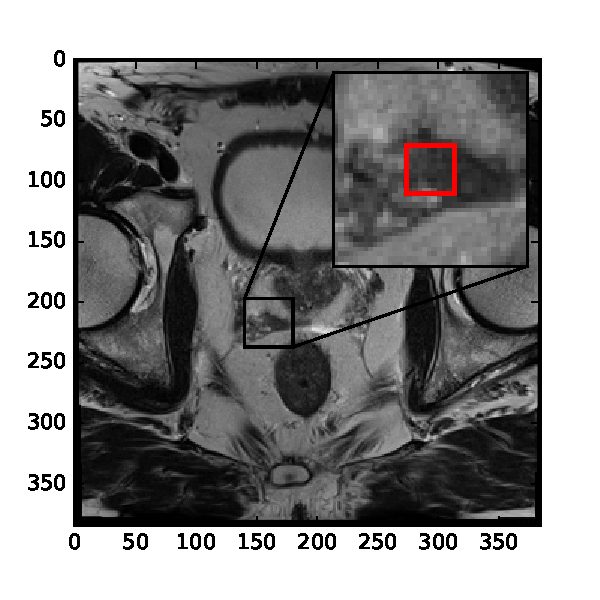
\includegraphics[]{figure-patch.pdf}
\end{center}
\end{figure}

\subsection{Normalization}

Each input dimension has the mean subtracted and is divided by the standard deviation. This ensures that the distribution of each dimension is approximately normal. $K^{\mathit{trans}}$ values are also transformed with a log function to correct for large skew.

\subsection{Example Weighting}

ProstateX training labels are highly unbalanced, with 76 positives and 254 negatives. It is necessary to weight the classes appropriately\cite{Yang2009}, the following formula is used:

\begin{equation}
\text{class weight} =
\frac
    {\text{total number of examples}}
    {\text{number of classes} \times \text{number of examples in class}}
\end{equation}
    
The positive class is given a weight of $ 330 / (2 \times 76) =  2.17 $ and negative class a weight of $ 330 / (2 \times 254) = 0.65 $. This can be interpreted as making it approximately three times worse to incorrectly label a positive case than a negative case during training.

\subsection{Kernel Selection}

The SVM kernel selected is the radial basis function (RBF); together called the RBF-SVM. This is a non-linear kernel so increases/decreases in one dimension do not necessarily cause proportional changes in score output. The authors believe that this is a desirable characteristic. Empirically, linear models also performed much worse and were abandoned early on.

\subsection{Hyperparameter Selection}

RBF-SVMs require tuning of two hyper-parameters a regularization parameter $C$ and a kernel parameter $\gamma$. The highest scoring settings achieved with 3-fold cross validation\cite{Hastie2009} (CV) are used. Final AUC is calculated by averaging AUC over every fold. A simple grid search is carried out, where each combination of $C \in \{0.1, 0.5, 1, 2, 5, 10, 20, 30, 50\}$ and $\gamma \in \{10^{-1}, 10^{-2}, 10^{-3}, 10^{-4}, 10^{-5}\}$ is scored and the best combination selected, see table \ref{table:performance} for selected values.

\subsection{Scoring}

The ProstateX challenge required entries to provide a continuous significance score for each test lesion, while SVMs produce a discrete binary classification. However a score can be easily derived for SVMs by using the decision function value directly instead of just the sign. This score increases in magnitude as the example moves further away from the SVM decision boundary. E.g. A score near zero indicates that small changes to this input would cause the prediction to change; while conversely, a large positive or negative value indicates that a small change in this input would not lead the prediction to change. Deriving the score in this way is practical and effective for this task.

\begin{table}
  \caption{Comparison of cross validation performance for differing configurations}
  \label{table:performance}

  \begin{center}
  \begin{tabular}{ l | r | r | r }
    & AUC  & C  & $\gamma$ \\
    \hline
    Image patch only    & .782 & 50 & $10^{-5}$  \\
    With zone           & .806 & 30 & $10^{-5}$  \\
    With class weights  & .811 & 30 & $10^{-3}$  \\
  \end{tabular}
  \end{center}
\end{table}

\subsection{Implementation}

This competition entry is reproducible and implemented using only open source software including Python, PyDICOM, SimpleITK\cite{simpleitk}, Scikit-Learn\cite{scikit-learn} and NumPy\cite{numpy}. Source code is available from the authors under an open source license.

\section{Alternative Approaches}

While the method descried here is self-contained, during development many different models and ideas were implemented and compared. Generally, multiple approaches were worked on in parallel. Ideas generated or problems encountered on one front would lead to progress on another. Some may be a path for future work.

\begin{description}
\item [Logistic regression\cite{Hastie2009}] was implemented based on several hand coded features and on features derived from fully-connected autoencoders and convolutional autoencoders\cite{hinton2006reducing}. But these methods never surpassed .75 AUC in cross validation.
\item [Convolutional neural networks\cite{NIPS2012_4824} (CNN)] were implemented, varying in depth from 3 to 20+ layers. Multiple architectures were tried including fully convolutional networks and residual networks. Generally it was very hard to prevent these large models from overfitting even with intense regularization and data augmentation. Models were heavily regularized using standard techniques, including dropout, gaussian activation noise and L2.
\item [Semi-supervised learning with Generative Adversarial Networks (GAN)\cite{salimans2016improved}] was implemented to try and augment the training data with the unlabeled test data. While GANs were able to generate high quality fake lesion images, the CV performance was disappointing, hovering around .65 AUC despite being an extensive and sophisticated model.
\item [Specialized data augmentation] was implemented. Extra synthetic data is generated by applying small modifications to existing data, for example, randomly cropping an area from an existing scan or generating a small random 3D rotation and resampling MRI scan data along new transformed axes. This technique gave a small performance increase for some neural network models.
\item [Extra metadata] including age, weight and sex was extracted from inside the training DICOM files and input into the model, this did seem to modestly increase performance in some circumstances. Although this extra metadata was not used in the final competition submission.
\end{description}

\section{DISCUSSION}

These results demonstrate that with care and correct application, well understood and reliable machine learning tools apply well to computer-aided diagnosis. It is empirically shown that relatively simple models can compete with more complex or heavily engineered models. While not the most accurate model, simplicity, flexibility and computational efficiency have their own benefits and may make this model much easier to certify and deploy in real-world environments.

% References
\bibliography{report} % bibliography data in report.bib
\bibliographystyle{spiebib} % makes bibtex use spiebib.bst

\end{document}
